\documentclass[a4paper,10pt]{report}

\topmargin -2cm
%\topskip0cm
%\footskip0cm
%\headsep0cm
\parindent0cm
\oddsidemargin -1cm
\evensidemargin -1cm
\headheight 2cm
\textheight 24cm
\textwidth 18cm

\author{Alexander M\"unn (4403061)}
\title{\"Ubung}

\include{tex/header}
\usepackage{fancyhdr}
\pagestyle{fancy}
\lhead{Michael Borst\\ Alex Muenn}
\chead{"Ubungsblatt \nr\\\today}
\rhead{Computer Vision}



\newcommand{\nr}{1}

\begin{document}
\section*{Aufgabe 1 - Bayer Filter und Demosaicing}

\begin{figure}[htpb]
\begin{center}
\subfigure[Eingabe Bild]{\includegraphics[width=0.25\textwidth]{samples/debug16}}
\subfigure[Bayer Bild]{\includegraphics[width=0.25\textwidth]{u01/debug16_bayer}}
\subfigure[Rekonstruktion]{\includegraphics[width=0.25\textwidth]{u01/debug16_dem}}
\end{center}
\caption{RGB - Bayer - RGB Transformation auf 16x16 Pixel Bild}
\label{fig:u01t1-debug}
\end{figure}

\lstset{language=matlab}
\begin{lstlisting}[caption={Bayer Transformation}]
  C = RGBImage;
  
  % G | B | G | B ...
  % R | G | R | G ...
  %
  % prepare red channel
  C(1:2:rows,:,1) = 0;
  C(2:2:rows, 2:2:cols, 1) = 0;
  % prepare blue channel
  C(2:2:rows,:,3) = 0;
  C(1:2:rows, 1:2:cols, 3) = 0;
  % prepare green channel
  C(1:2:rows, 2:2:cols, 2) = 0;
  C(2:2:rows, 1:2:cols, 2) = 0;

  Out = C(:,:,1) + C(:,:,2) + C(:,:,3);
\end{lstlisting}

\begin{lstlisting}[caption=R\"ucktransformation von Bayer nach RGB]
  B = I_bayer;
% apply a kernel in current global position row r and column c of bayer image B
  function v = apply(K)
    global B r c
    % determine kernel size
    [rowsK, colsK] = size(K);
    % create 'view matrix' according to kernel size
    rFrom = r-floor(rowsK/2);
    cFrom = c-floor(colsK/2);
    Sub = B(rFrom:rFrom+rowsK-1,cFrom:cFrom+colsK-1);

    v = sum(sum(Sub.*K));
  end
%-------------------------------------------------------------------------------
% Kernel definitions:
  G_at_R = [ 0  0 -1  0  0
             0  0  2  0  0
            -1  2  4  2 -1
             0  0  2  0  0
             0  0 -1  0  0];
  G_at_R /= 8;
  G_at_B = G_at_R;
  
  R_at_G_in_Rrow_Bcol  = [ 0  0 0.5 0  0
                           0 -1  0 -1  0
                          -1  4  5  4 -1
                           0 -1  0 -1  0
                           0  0 0.5 0  0]* 1/8;
  R_at_G_in_Brow_Rcol = R_at_G_in_Rrow_Bcol';
  B_at_G_in_Brow_Rcol = R_at_G_in_Rrow_Bcol;
  B_at_G_in_Rrow_Bcol = R_at_G_in_Brow_Rcol;
  R_at_B = [ 0   0 -3/2  0   0
             0   2   0   2   0
            -3/2 0   6   0 -3/2
             0   2   0   2   0
             0   0 -3/2  0   0]*1/8;
  B_at_R = R_at_B;
%-------------------------------------------------------------------------------
  for r = 3:(rows-2)
    for c = 3:(cols-2)
      % first: copy 
      
      % red row
      if mod(r,2) == 0
        if mod(c,2) == 0
          % red row, blue column
          I_rgb(r,c,green) = I_bayer(r,c);
          I_rgb(r,c,red) = apply(R_at_G_in_Rrow_Bcol);
          I_rgb(r,c,blue) = apply(B_at_G_in_Rrow_Bcol);
        else
          % red row, red column
          I_rgb(r,c,red) = I_bayer(r,c);
          I_rgb(r,c,green) = apply(G_at_R);
          I_rgb(r,c,blue) = apply(B_at_R);
        end
      % blue row
      else 
        if mod(c,2) == 0
          % blue row, blue column
          I_rgb(r,c,blue) = I_bayer(r,c);
          I_rgb(r,c,green) = apply(G_at_B);
          I_rgb(r,c,red) = apply(R_at_B);
        else
          % blue row, red column
          I_rgb(r,c,green) = I_bayer(r,c);
          I_rgb(r,c,red) = apply(R_at_G_in_Brow_Rcol);
          I_rgb(r,c,blue) = apply(B_at_G_in_Brow_Rcol);
        end
      end
    end
  end
\end{lstlisting}


\begin{figure}[htpb]
\begin{center}
\subfigure[Eingabe Bild]{\includegraphics[width=0.25\textwidth]{samples/lenna512c}}
\subfigure[Bayer Bild]{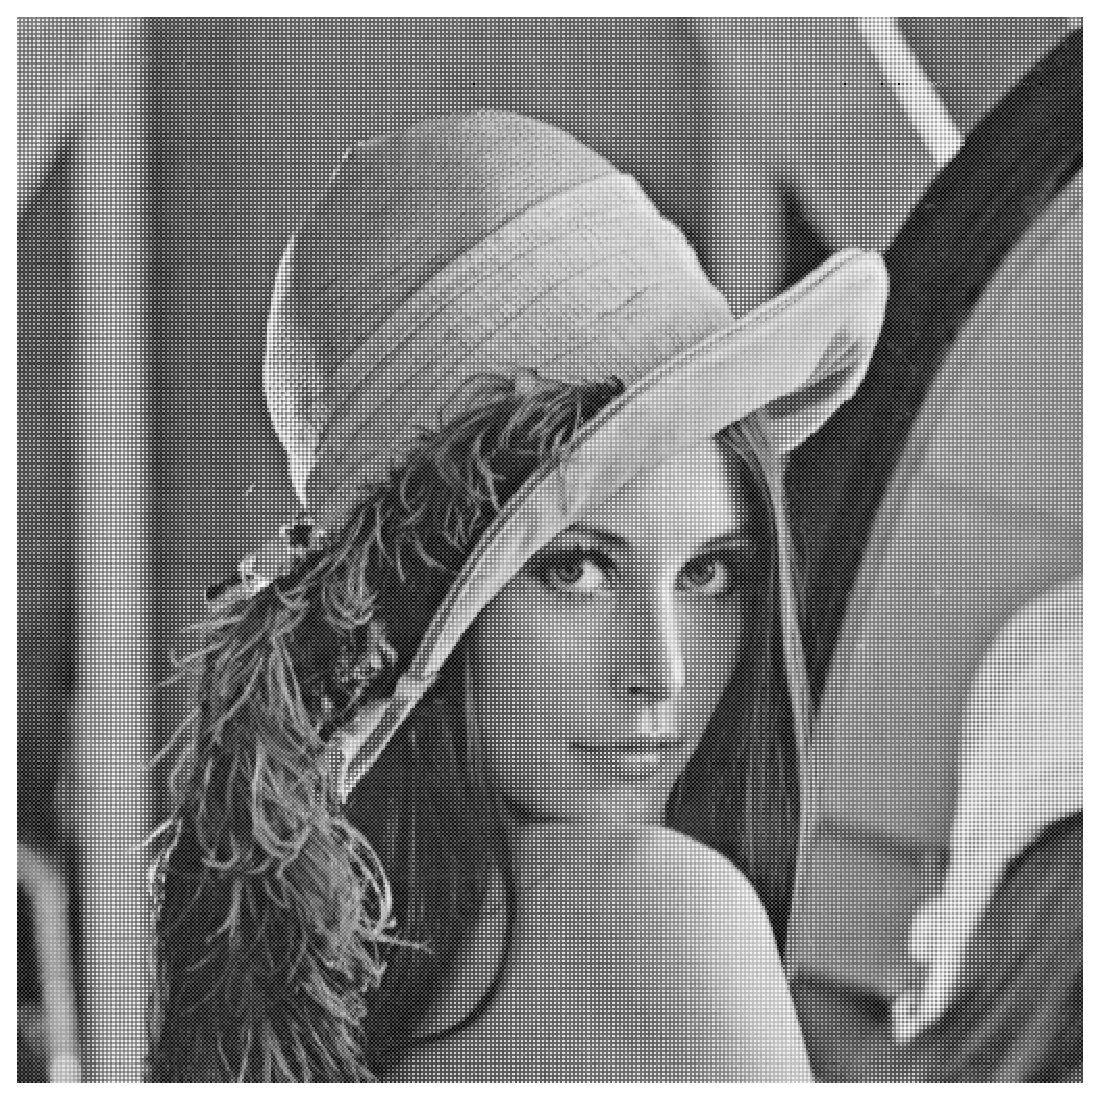
\includegraphics[width=0.25\textwidth]{u01/lenna512c_bayer}}
\subfigure[Rekonstruktion]{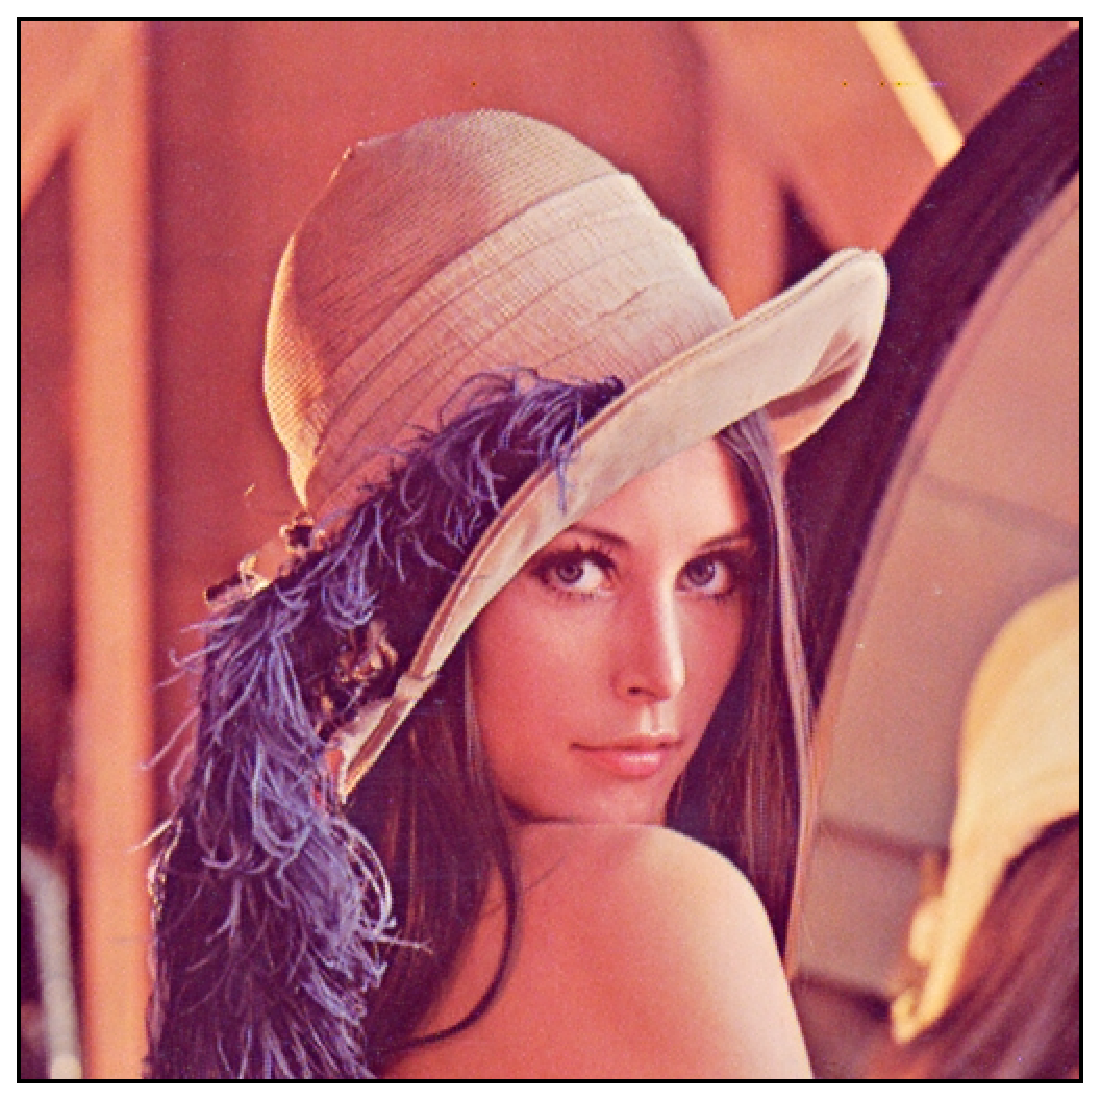
\includegraphics[width=0.25\textwidth]{u01/lenna512c_dem}}
\end{center}
\caption{RGB - Bayer - RGB Transformation auf ``Lenna''}
\label{fig:u01t1-lenna}
\end{figure}

Im Vergleich zu Abbildung~\ref{fig:u01t1-debug} sind in Abbildung~\ref{fig:u01t1-lenna} 
kaum bis keine Rekonstruktionsartefakte zu erkennen. Die l\"asst sich damit erkl\"aren,
dass unser gew\"ahltes Interpolationsverfahren zwar Kanten ber\"ucksichtigt, aber an
scharfen Farb\"uberg\"angen scheitert.

\section*{Aufgabe 2 - UV-Histogramm} 


% \includegraphics[width=150mm]{<file.eps>}
\end{document}
